\documentclass[svgnames,x11names,tikz]{standalone}
\usepackage{xcolor}
\usetikzlibrary{arrows,positioning,backgrounds,fit}

\begin{document}
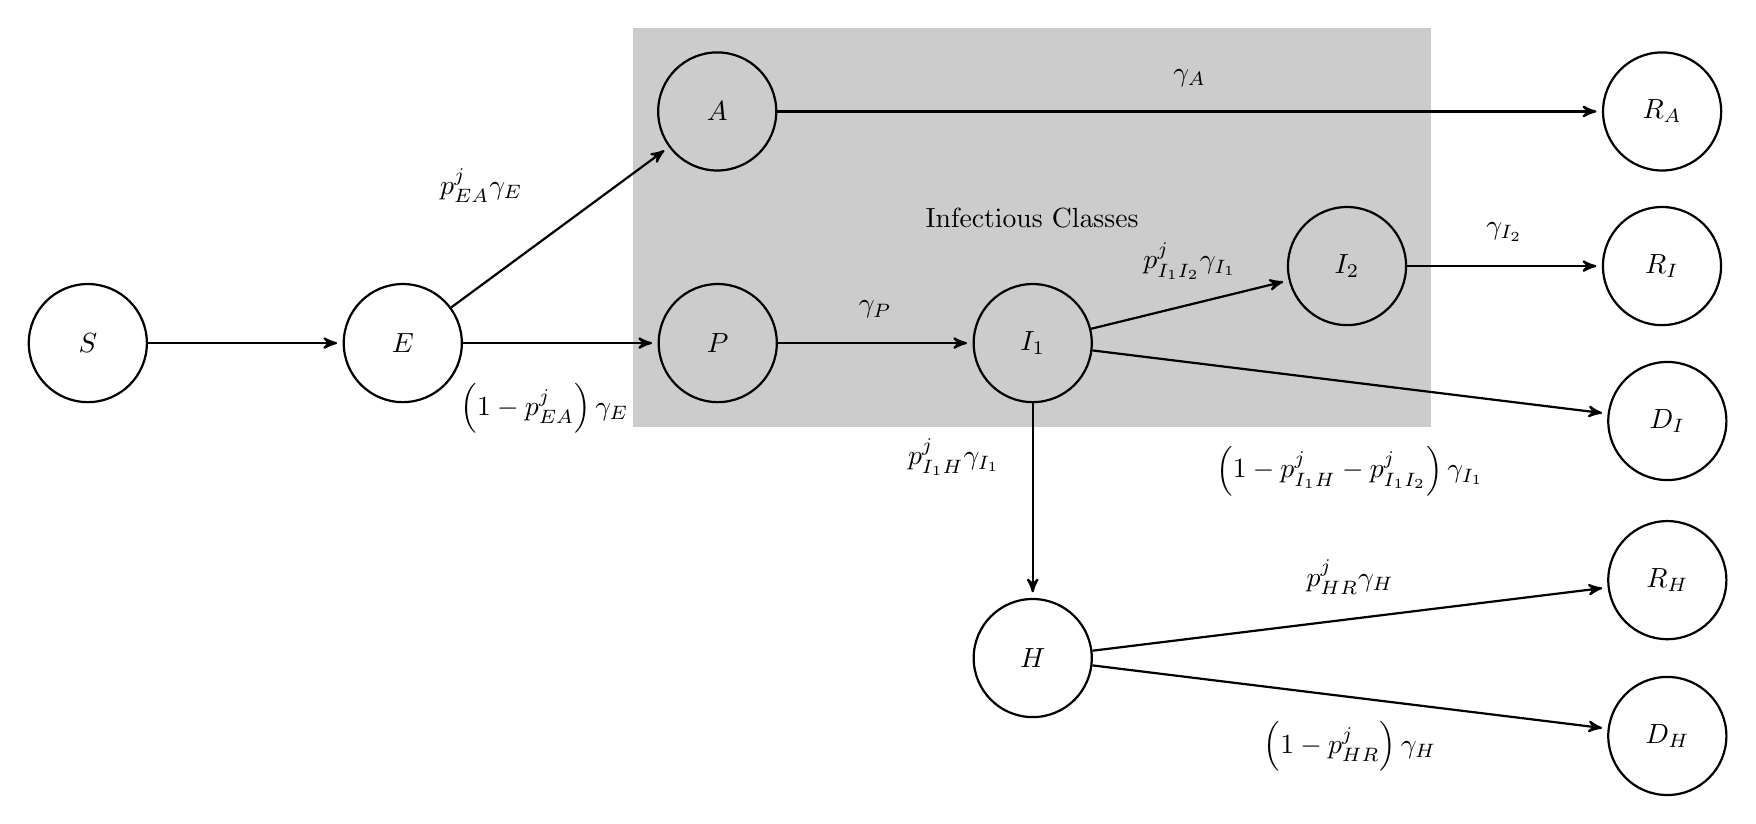
\begin{tikzpicture}[, >=stealth', inner sep = 3mm, thick]
	\tikzstyle{comp} = [circle, draw = black, minimum size = 1.5cm]
	\tikzstyle{demo} = [rectangle, draw = black, minimum size = 1.5cm]
    \begin{scope}[node distance = 4cm]
	    \node [comp] (S) {$S$};
	    \node [comp] (E) [right of = S] {$E$};
      \node [comp] (A) at ([shift=({36.38:4.96cm})]E) {$A$};
      \node [comp] (RA) [right of = A, node distance = 12cm] {$R_A$};
      \node [comp] (P)  [right of = E] {$P$};
      \node [comp] (I1) [right of = P] {$I_1$};
      \node [comp] (I2) at ([shift=({13.77:4.11cm})]I1) {$I_2$};
      \node [comp] (RI) [right of = I2] {$R_I$};
      \node [comp] (DI) at ([shift=({-7:8.12cm})]I1) {$D_I$};
      \node [comp] (H) [below of = I1] {$H$};
      \node [comp] (RH) at ([shift=({7:8.12cm})]H) {$R_H$};
      \node [comp] (DH) at ([shift=({-7:8.12cm})]H) {$D_H$};
	    \draw [->, shorten >=2pt] (S) -- (E);	
      \draw [->, shorten >=2pt] (E) -- node [below, xshift = -0.2cm, yshift = -0.2cm] {$\left(1 - p_{EA}^j\right) \gamma_E$} (P);
      \draw [->, shorten >=2pt] (E) -- node [above, xshift = -1cm] {$p_{EA}^j \gamma_E$} (A);
      \draw [->, shorten >=2pt] (A) -- node [above] {$\gamma_A$} (RA);
      \draw [->, shorten >=2pt] (P) -- node [above] {$\gamma_P$} (I1);
      \draw [->, shorten >=2pt] (I1) -- node [above] {$p_{I_1I_2}^j\gamma_{I_1}$} (I2);
      \draw [->, shorten >=2pt] (I1) -- node [above, xshift = -1cm] {$p_{I_1H}^j\gamma_{I_1}$} (H);
      \draw [->, shorten >=2pt] (I2) -- node [above] {$\gamma_{I_2}$} (RI);
      \draw [->, shorten >=2pt] (I1) -- node [below, yshift = -0.5cm] {$\left(1 - p_{I_1H}^j - p_{I_1I_2}^j\right)\gamma_{I_1}$} (DI);
      \draw [->, shorten >=2pt] (H) -- node [above] {$p_{HR}^j\gamma_{H}$} (RH);
      \draw [->, shorten >=2pt] (H) -- node [below] {$\left(1 - p_{HR}^j\right)\gamma_{H}$} (DH);
      \scoped[on background layer]{\node [fit=(A)(P)(I1)(I2), fill = black!20] {Infectious Classes};}
    \end{scope}
\end{tikzpicture}
\end{document}